\subsection{Client - Java}
\label{sec:Javaclient}

Der hier beschriebene Javaclient ist ein möglicher Teilnehmer, der sich mit den Kommunikationsserver verbinden und ein Spiel austragen kann.
Sein Design orientiert sich am Model-View-Controller Prinzip, wobei das Spielbrettmodell auf Grund seines geringen Umfangs im Controller eingebettet wurde.

Eine Übersicht des Entwurfs wird in Abbildung \ref{fig:Javaclientklassendiagramm} dargestellt.


\begin{figure}[H]
  \centering
  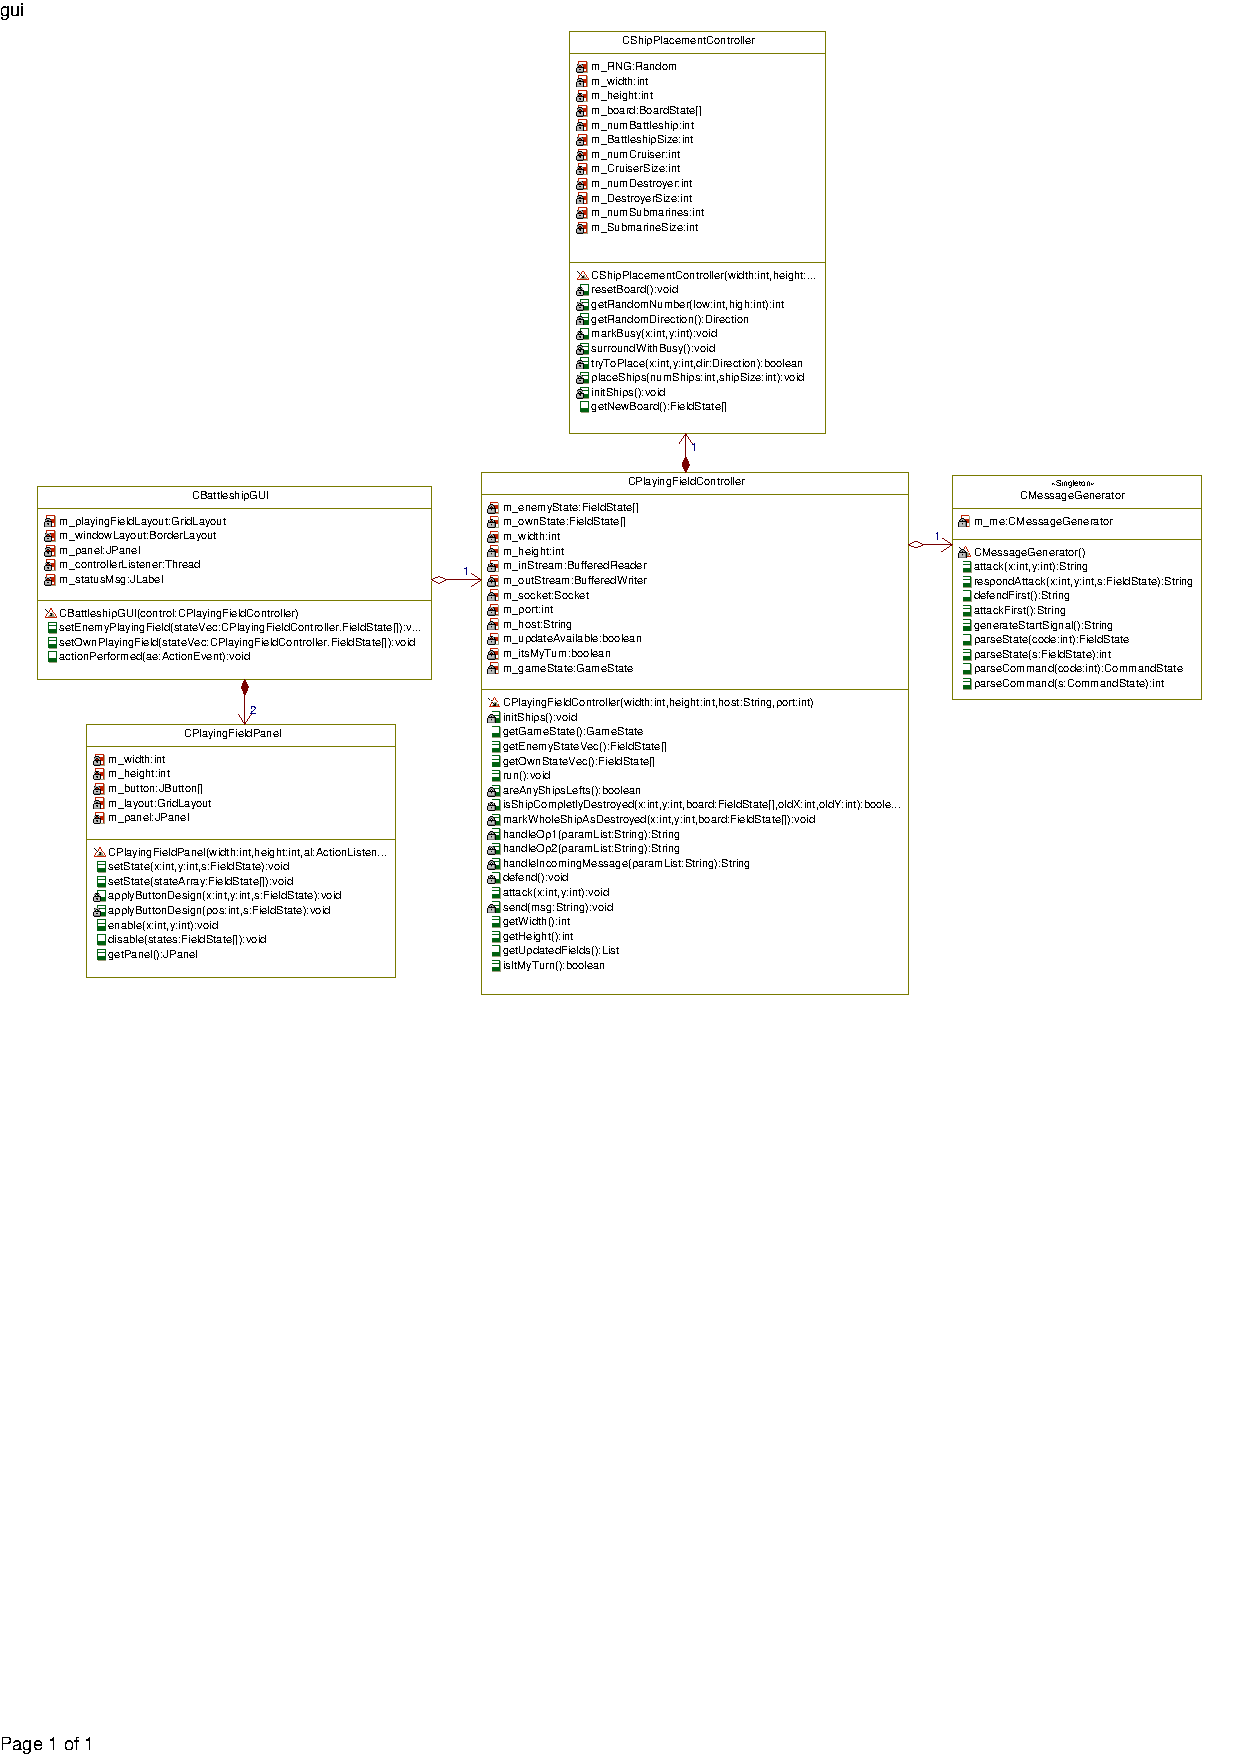
\includegraphics[trim=5mm 125mm 5mm 4mm,clip,width=0.9\textwidth]{images/CJavaClient.pdf}
  \caption{Klassendiagramm des Java Clients}
  \label{fig:Javaclientklassendiagramm}
\end{figure}
